% !TEX root = main.tex

% options:
% thesis=B bachelor's thesis
% thesis=M master's thesis
% czech thesis in Czech language
% slovak thesis in Slovak language
% english thesis in English language
% hidelinks remove colour boxes around hyperlinks

\documentclass[thesis=B,english]{FITthesis}[2012/06/26]

\usepackage[utf8]{inputenc} % LaTeX source encoded as UTF-8

\usepackage{graphicx} %graphics files inclusion
\usepackage{amsmath} %advanced maths
% \usepackage{amssymb} %additional math symbols
\usepackage{dirtree} %directory tree visualisation
\usepackage{cleveref}
\usepackage{hyperref}
% % list of acronyms
\usepackage[acronym,nonumberlist,toc,numberedsection=autolabel]{glossaries}
\iflanguage{czech}{\renewcommand*{\acronymname}{Seznam pou{\v z}it{\' y}ch zkratek}}{}
\makeglossaries

%\newcommand{\tg}{\mathop{\mathrm{tg}}} %cesky tangens
%\newcommand{\cotg}{\mathop{\mathrm{cotg}}} %cesky cotangens

% following 3 commands (todo, tmp image) Used from http://www.herout.net/blog/2017/03/pomalu-uz-pojdme-psat/
\usepackage{xcolor} 
\newcommand{\todo}[1]{\textcolor{red}{\textbf{[#1]}}}

\usepackage{blindtext}
\newcommand{\blind}[1][1]{\textcolor{gray}{\Blindtext[#1][1]}}

\setlength{\fboxsep}{0.005pt}
\newcommand{\tmpframe}[1]{\fbox{#1}}
%\renewcommand{\tmpframe}[1]{#1}  % uncomment before production

% % % % % % % % % % % % % % % % % % % % % % % % % % % % % % 

\department{Department of software engineering science}
\title{Mobile Enterprise Architecture Process Analytic Tool Based on the DEMO Methodology}
\authorGN{Petr} %(křestní) jméno (jména) autora
\authorFN{Nymsa} %příjmení autora
\authorWithDegrees{Petr Nymsa} %jméno autora včetně současných akademických titulů
\author{Petr Nymsa} %jméno autora bez akademických titulů
\supervisor{Ing. Marek Skotnica}
\acknowledgements{Doplňte, máte-li komu a za co děkovat. V~opačném případě úplně odstraňte tento příkaz.}
\abstractCS{
% Tato bp se zabývá (řeší)...
% Cílem práce je
% V práci se zaměřuji na
% Literární rešerše se zabývá...praktická část práce navazuje...
Cílem této práce je vytvoření metody vizualizace procesů založených na metodice DEMO. Kromě vizualice jsou rozebrány možnosti sběru dat z těchto procesů a následná jejich analýza a grafické znázornění. V práci je popsána metodika DEMO a čím se liší od systémů, které využívají notaci BPM. Pro ověření vymyšleného konceptu je vypracována ukázková implementace jako mobilní aplikace, která umožní vizualizovat procesy na modelovém příkladu. 

% čím je práce užitečná
}
\abstractEN{Sem doplňte ekvivalent abstraktu Vaší práce v~angličtině.}
\placeForDeclarationOfAuthenticity{V~Praze}
\declarationOfAuthenticityOption{4} %volba Prohlášení (číslo 1-6)

\keywordsCS{mobilní aplikace, vizualizace procesů, DEMO, analýza dat, business intelligence, podnikové inženýrství, procesní řízení, BPM, Xamarin}

\keywordsEN{mobile application, business intelligence, DEMO, enterprise engineering, business process management, BPM, analytic tool, Xamarin}
% \website{http://site.example/thesis} %volitelná URL práce, objeví se v tiráži - úplně odstraňte, nemáte-li URL práce

\begin{document}

% \newacronym{CVUT}{{\v C}VUT}{{\v C}esk{\' e} vysok{\' e} u{\v c}en{\' i} technick{\' e} v Praze}
% \newacronym{FIT}{FIT}{Fakulta informa{\v c}n{\' i}ch technologi{\' i}}

\newglossaryentry{formula}
{
        name=formula,
        description={A mathematical expression}
}

\newacronym{dwma}{DWMA}{DEMO WIP Mobile Application}
\newacronym{rac}{RAC}{Rent-A-Car}
\newacronym{eo}{EO}{Enterprise Ontology}
\newacronym{demo}{DEMO}{Design and Engineering Methodology for Organizations}
\newacronym{ocd}{OCD}{Organization Construction Diagram}
\newacronym{psd}{PSD}{Process Structure Diagram}
\newacronym{kpi}{KPI}{Key Performance Indicator}
\newacronym{bpm}{BPM}{Business Process Management}
\newacronym{bpmn}{BPMN}{Business Process Model and Notation}
\newacronym{bpms}{BPMS}{Business Process Model Systems}

\begin{introduction}
	Nowadays almost every company has more independent systems which can help employees to do their job. For example one system for accountancy, another for warehouses and another one for managing orders or something similar. However how business grows, some kind of business analysis is required. Usually some person is instructed to analyse the business, how to make it better. The person collects all required data from every system, typically in some form of  ``Excel table'' and over it he does analysis. This approach at the beginning can be sufficient, however sooner or later, it will become heavy, uncomfortable and mainly not effective way how to do this kind of analysis. All required data are spread over all systems without any order. Some systems can have functions to export data in some suitable form, but from another systems they can export data only in some form of plain-text and so on.  At some point people find out that in their business ``reigns chaos''. Fortunately this ``chaos'' can be controlled with some well known approaches. Most well known term of how ``chaos' can be controlled is Business Process Management (BPM).

\section{Analysis within BPM}
Every task or set of tasks within the business can be formulated as \textit{business process}. For example task ``Order of new components for machine'' (which consists of many additional steps)  can be expressed as business process ``New machine components order''. The well-defined business processes are the first step to having better control over own business and also for further analysis. 

Next step is that these defined processes connect under one system with internal business applications. The ``one system'' is typically marked as BPM System (BPMS). Within BPMS the business processes are defined, modelled and executed. Modelling is typically done through Business Process Model and Notation (BPMN) which is a well-known method to model business processes. Execution means, that dependent internal systems within business communicates with BPMS and output from these systems is reflected in BPMS. This is the second important step to have a more precise analysis of own business.

If the company has some kind of BPMS, they have also well-defined data and aggregated them in one place. Usually, every BPMS offers functionalities to do analysis and monitoring over collected data. These functionalities can help people managing their business, more easily finding issues and potentially solving them. Monitoring is typically done through graphical overviews, which offer varied views on the business metrics. These metrics can be for example business efficiency, employee performance (how much the desired goals are fulfilled), financial efficiency and so on. Thanks to these systems people have the better understanding of their business and they can more easily focus on the critical places that can be improved.

\section{A New Approach}
While BPMN is well known and widely used, the new methodology was introduced by \textit{J.Dietz}~\cite{dietz-essence-2015}. This new methodology called DEMO is considered as successor of BPMN. DEMO is build on high-quality scientific foundations, which brings against BPMN (and similar methods) better modelling of business processes. Although DEMO is well defined methodology, BPMS based on DEMO does not (nearly) exists. The problem of BPMS based on DEMO is subject of many researches. There are first attempts to achieve a solution based on DEMO, which can design processes and execute them. However the monitoring and analysis are missing.

This thesis focuses on visualisation of business processes based on DEMO methodology. Within defined process the goal of thesis is to find a way:

\begin{itemize}
\item The data processing from internal systems and their connection within DEMO model. 
\item Offer data to users with appropriate graphical overviews.
\item Real-time visualisation of running processes.
\end{itemize}

\section{Motivation}
The main reason why I have focused on this topic comes from a school project. With our team we created chatbot application for pizza delivering system which was based on DEMO methodology. In fact we used \textit{DEMO Engine}, the BPMS based on DEMO developed by \textit{ForMetis} company\todo{citation needed}. Moreover, on this \textit{DEMO Engine} worked also my supervisor (and also the team leader of our team) \textit{M.Skotnica}~\cite{diploma-skotnica-2016}. Within \textit{engine} we defined model for ``imaginary'' pizzeria. Then we used this defined processes and connected them with the chatbot. However, this system had only ability to design, model and execute processes. The monitoring of collected data or visualisation of processes were missed. That's why I have chosen this topic.

\section{Structure}
The thesis is divided to four chapters:
\begin{itemize}
\item In \cref{ch:theoretical-foundations} underlying theories and terms are explained.
\item In \cref{ch:bpms} research of existing BPMS solutions follows. Then some specific solutions are investigated for analysis of own solution. Role of DEMO within BPMS is described. 
\item Then in \cref{ch:proposed-approach} the proposed approach is introduced. The theory and research from previous chapters are used. The concept of a system is described. Principle of real-time visualisation is more precisely explained. 
\item In \cref{ch:proof-of-concept} implementation of proof-of-concept is created. Architecture and used technologies are described. An example model of business processes is demonstrated.
\end{itemize}
In conclusion the results are compared with the goals of this thesis. 




    
\end{introduction}

\chapter{The Theoretical Foundations}
\label{ch:theoretical-foundations}

In the first chapter, theoretical foundations are described. Firstly, terms such as BPM, Business Intelligence are explained. Then, the theory of Enterprise Ontology and DEMO methodology follow. In the end, Gantt chart is described, because it is used as part of visualisation approach. 
% -------------------------------------------------------------------------------
\section{Business Process Management}
\gls{bpm} is an approach that focuses on modelling, analysing, improving and monitoring business processes. 
The \gls{bpm} life-cycle can be divided to five stages as shown in \cref{fig:bpm-lifecycle}:

\begin{figure}[ht!]
	\centering
    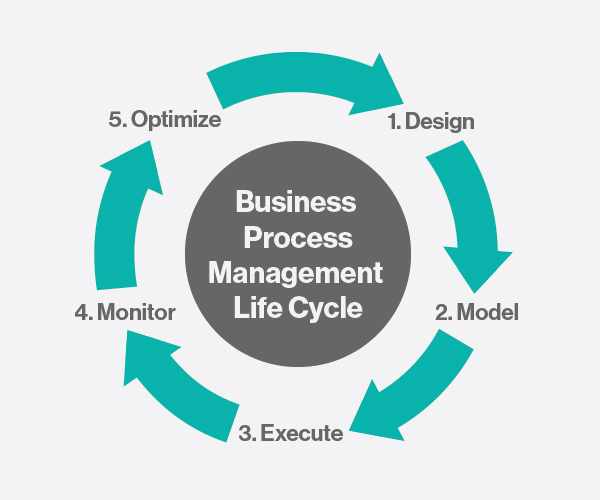
\includegraphics[width=0.6\textwidth, keepaspectratio]{img/bpm-lifecycle.jpg}
    \caption{BPM Life-cycle \cite{harvey-koeppel-bpm-lifecycle-2015}}
    \label{fig:bpm-lifecycle}
\end{figure}

\begin{description}
	\item[Design] -- The requirements of the business are collected, analysed and specified. The specification can be ``as is'' (state of how processes currently are) or ``to be'' (how processes would be). Accompanying graphical materials (such as flow-charts) are included.
    \item[Model] -- Specification is expressed (modelled) with graphical notation \gls{bpmn}, which will be investigated later.
    \item[Execute] -- Changes are implemented and deployed.
    \item[Monitor] -- After deployed changes, monitoring system comes to the scene. Processes are monitored and \gls{bpms} tools are used to collect data and analyse performance through metrics - called \gls{kpi}. \gls{kpi} are defined, optimized metrics which can help to understand the performance of the current business. As an example of \gls{kpi} can be ``an average number of requests for new order per day'' and many more, individual metrics to concrete business.
    \item[Optimize] -- At some point, when an appropriate number of data are collected and analysed with monitoring, optimization is done. The goal of optimization is to find issues or some improvements. After that, new specifications and improvements are created and \textit{design} stage is executed again.
\end{description}
% -------------------------------------------------------------------------------
\subsection{Business Process Model and Notation}
\gls{bpmn} is notation created and standardised by \textit{Object Management Group} (see \url{https://www.omg.org}). According to~\cite{bpmn-org-2018} \gls{bpmn} can be described as:
\begin{quote}
  \gls{bpmn} is a graphical notation that depicts the steps in a business process. BPMN depicts the end to end flow of a business process. The notation has been specifically designed to coordinate the sequence of processes and the messages that flow between different process participants in a related set of activities.
\end{quote}
The notation itself, elements which are used and how modelling is done, are not described. For this information, see~\cite{bpmn-org-2018}.
% -------------------------------------------------------------------------------
\section{Business Intelligence}

\gls{bi} is a way how business can collect an enormous amount of data, structure them and analyse (see \cref{fig:bi-diagram}. From \gls{bpm} life-cycle view, \gls{bi} is a \textit{Monitor} stage. Systems which are tagged as \gls{bi} tools typically offers some kind of reporting, dashboards and scorecards. 

\begin{figure}[ht!]
	\centering
    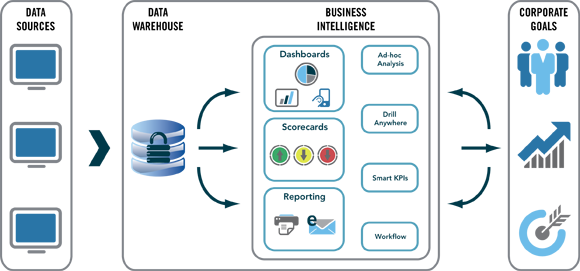
\includegraphics[width=0.6\textwidth]{img/mortgage-business-intelligence-diagram.png}
    \caption{Business intelligence diagram \cite{business-intelligence-diagram-2018}}
    \label{fig:bi-diagram}
\end{figure}

\textbf{Dashboard} offers graphical overviews of collected data. Dashboards are typically highly customizable and can offer different types of views for each employee to help achieve their job. Dashboards can help understand and find issues within business and potentially more quickly solve them. \Cref{fig:bi-dashboard} shows an example. 

\textbf{Scorecards} offer monitoring of \gls{kpi} metrics and user can easy compare goals and current results. Scorecards also easily show performance of business, for example if business plan is fulfilled or financial flow (e.g if business is profiting or not,\dots). 

\begin{figure}[ht!]
	\centering
    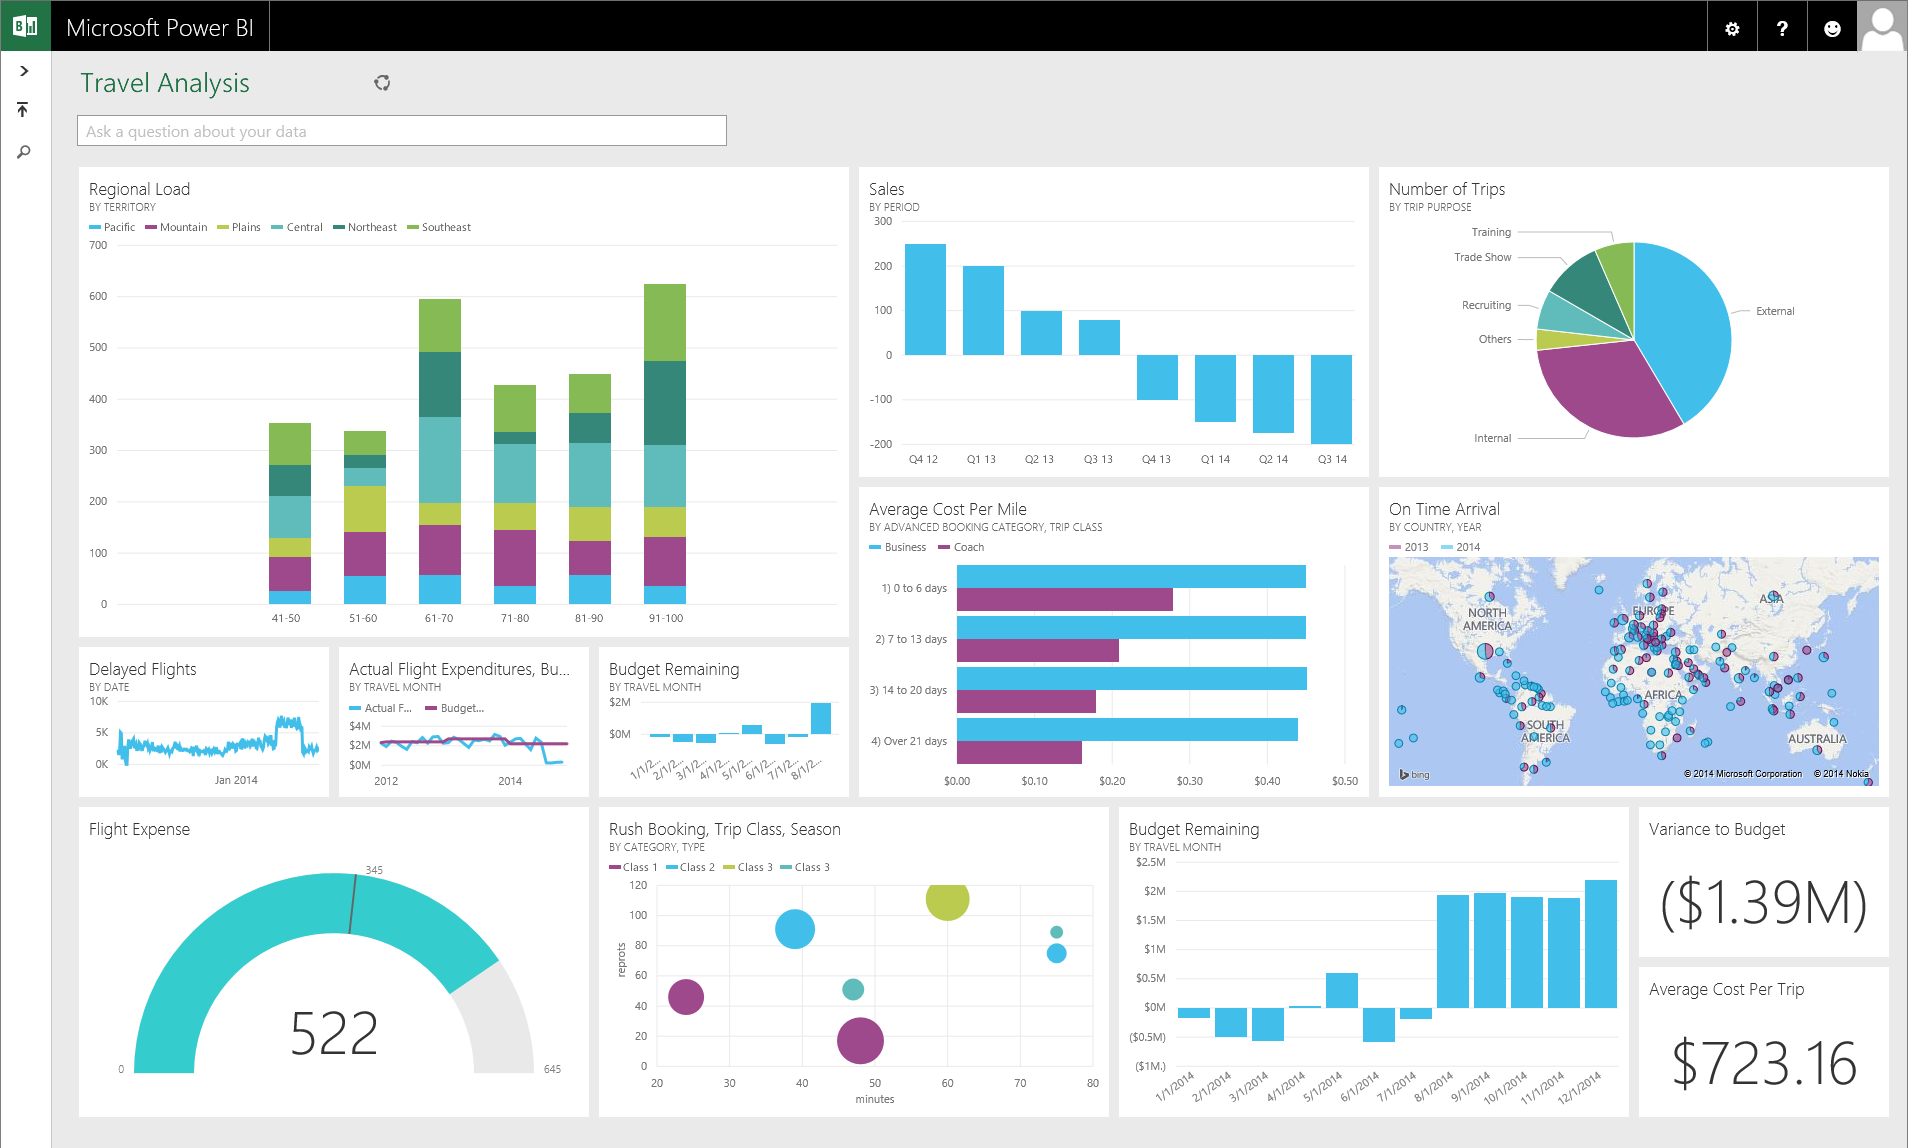
\includegraphics[width=0.6\textwidth]{img/microsoft-power-bi-dashboard.png}
    \caption{Business Intelligence dashboard example~\cite{ms-business-intelligence-2018}}
    \label{fig:bi-dashboard}
\end{figure}
% -------------------------------------------------------------------------------
\section{Enterprise ontology}
According to~\cite{gruber-translation-1993}, definition of ontology states as ``An ontology is a specification of a conceptualization''. In other words ontology is description, a formal specification, of concepts and relationships.

Enterprise Ontology~\cite{dietz-essence-2015} is the understanding of the essence of organisation, completely independent of the way in which this essence is realised and implemented.

The DEMO Methodology~\cite{dietz-enterprise-2006} is an engineering methodology, based on theory of enterprise ontology.

The following text was taken from article describing \gls{eo} theory~\cite{haan-modeling-2009}:

\begin{quotation}
Enterprise ontology is focused on the essence of the operation of an organization, meaning that it is fully independent of the (current) realization and implementation of the organization. The theory that underlies the notion of enterprise ontology as presented by Dietz is called the PSI-theory. Dietz uses this theory to construct a methodology providing an ontological model of an organization, i.e. a model that is coherent, comprehensive, consistent, and concise, and that only shows the essence of the operation of an organization model. This methodology is called \gls{demo}.

Compared to its implementation model, the ontological model of an enterprise offers a reduction of complexity of over 90\%. This reduction of complexity makes an organization for a manager intellectual manageable and transparent. It also shows the coherence between all fields within the enterprise, like business processes, workflow, organization structure, etc.

The overall goal of the PSI-theory (the theory behind the notion of Enterprise Ontology) is to extract the essence of an organization from its actual appearance. It presents four axioms that help to achieve this goal.

The \textbf{operation axiom} (\cref{fig:OperationAxiom}) tells us that the implementation independent essence of an organization is that it consists of subjects fulfilling actor roles. A subject fulfilling a certain actor role is called an actor. Actors constitute the operation of an organization by performing two kinds of acts: production acts and coordination acts.

\begin{figure}[ht!]
	\centering
    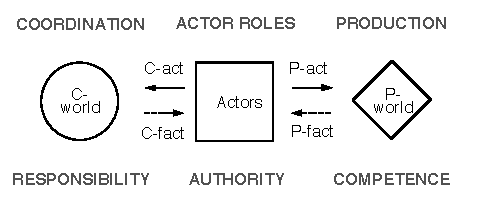
\includegraphics[width=10cm, keepaspectratio]{img/OperationAxiom}
    \caption{The operation axiom \cite{haan-modeling-2009}}
    \label{fig:OperationAxiom}
\end{figure}

By performing production acts (P-acts for short) the subjects contribute to bringing about the goods and/or services that are delivered to the environment of the organization. The results of P-acts are production facts (P-facts for short), which can be divided into material (something is manufactured, stored or transported) and immaterial (decisions or judgements) facts.

By performing coordination acts (C-acts for short) subjects enter into and comply with commitments towards each other regarding the performance of production acts. A C-act is performed by one actor, the performer, and directed to another actor, the addressee. C-acts consist of an intention (e.g. request, promise, question, assertion) and a proposition (the performer proclaims the fact and the associated time the intention is about) and result in coordination facts (C-facts for short).

The \textbf{transaction axiom} tells us that C-acts are performed as steps in universal patterns, called transactions. This axiom reveals universal socionomic patterns of coordination that hold for all organizations. The standard transaction pattern is shown in~ \cref{fig:TransactionPattern}. A white box represents a C-act type and a white disk represents a C-fact type. A gray box represents a P-act type and a gray diamond a P-fact type. 

\begin{figure}[ht!] 
	\centering
    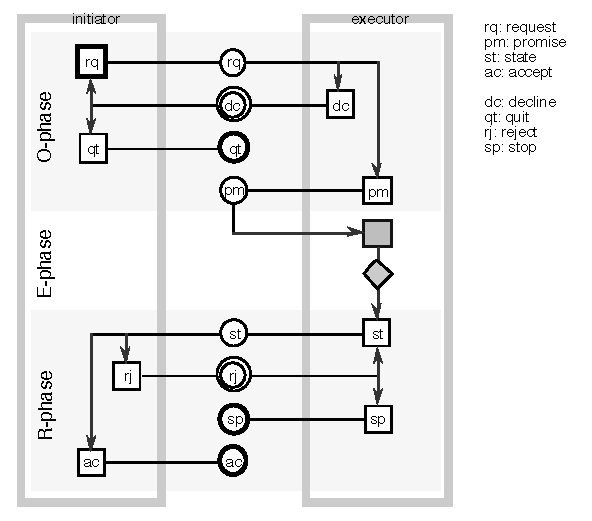
\includegraphics[width=8cm, keepaspectratio]{img/TransactionPattern}    
    \caption{The standard transaction pattern \cite{haan-modeling-2009}}
    \label{fig:TransactionPattern}
\end{figure}

Two actors are involved in a transaction, the initiator and the executor. A transaction evolves in three phases: the order phase (O-phase for short), the execution phase (E-phase for short), and the result phase (R-phase for short).

The \textbf{composition axiom} tells us how P-facts are interrelated. It states that every transaction is enclosed in some other transaction, or is a customer transaction of the organization under consideration, or is a self-activation transaction. According to Dietz this axiom provides the basis for a well-founded definition of the notion of business process.

The \textbf{distinction axiom} (\cref{fig:DisctinctionAxiom}) tells us that actors exert three basic human abilities: performa, informa, and forma. Through the distinction axiom a substantial reduction of complexity and diversity is achieved, regarding both the coordination and the production in an organization.

\begin{figure}[ht!]
	\centering
    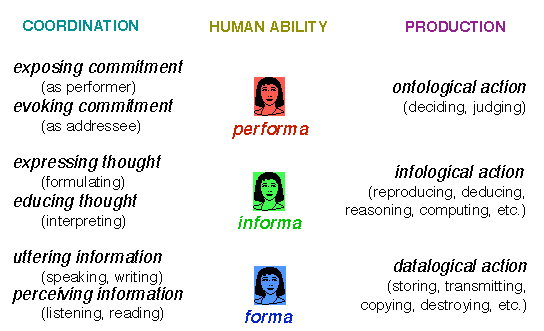
\includegraphics[width=10cm, keepaspectratio]{img/DistinctionAxiom}
    \caption{The distinction axiom \cite{haan-modeling-2009}}
    \label{fig:DisctinctionAxiom}
\end{figure}
% -------------------------------------------------------------------------------
\subsection{The Organization Theorem}

The organization theorem combines the benefits of these axioms into one concise, comprehensive, coherent, and consistent notion of enterprise. This theorem states that the organization of an enterprise is a heterogeneous system that is constituted as the layered integration of three homogeneous systems: the B-organization (from Business), the I-organization (from Intellect), and the D-organization (from Document). Figure~ \ref{fig:OrganizationPyramid} visualizes the organization theorem and shows us that the D-organization supports the I-organization, which supports the B-organization. The coordination parts of these three systems are similar, they only differ in the kind of production: the production of the B-organization is ontological, the production in the I-organization is infological, and the production in the D-organization is datalogical.

\begin{figure}[ht!]
	\centering
    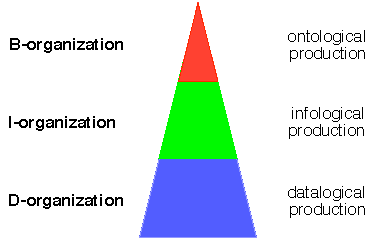
\includegraphics[width=6cm, keepaspectratio]{img/OrganizationPyramid}
    \caption{The organization theorem \cite{haan-modeling-2009}}
    \label{fig:OrganizationPyramid}
\end{figure}

\end{quotation}
% -------------------------------------------------------------------------------
\section{Modelling with DEMO}
In this section, firstly short description of modelling aspects is provided and then a illustrative example how modelling with \gls{demo} can be more precise and shorter than creating model with \gls{bpmn}. 

All used elements in DEMO modelling are described in aspects models arranged as pyramid. However the two core elements are Ontological transaction and Actor roles. Good summarization of these two core elements are from master thesis by Zuzana Vejrazkova~\cite{vejrazkova-demo-2013}:

\begin{quote}
	\begin{description}
		\item[Ontological transaction] -- Involves actions that happen on the ontological level, as described by the Distinction axiom. Those involve bringing about the facts that did not exist before, making decisions, or transporting physical elements. Completion of a transaction, in a way that is described by the transaction axiom, results in a new original fact, called the P-fact.
        \item[Actor role] -- There are two actor roles, the initiator and the executor. They play an important role in DEMO modelling, as each transaction needs to have exactly one initiator and one executor. On the implementation level, 1~person can (and often does) posses more actor roles.
	\end{description}
\end{quote}

Figure \ref{fig:DemoAspectModels} shows that ontological model can be divided to four sub-models. The good and brief explanation is in the book \textit{The essence of organisation: an introduction to enterprise engineering}~\cite{dietz-essence-2015}:

\begin{figure}[ht!]
	\centering
    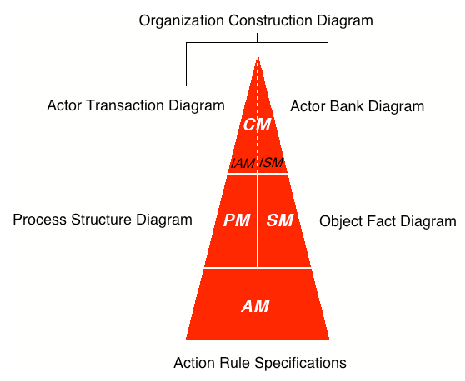
\includegraphics[width=8cm, keepaspectratio]{img/DemoAspectModels}
    \caption{The DEMO Aspect Models pyramid \cite{dietz-discipline-2013}}
    \label{fig:DemoAspectModels}
\end{figure}

\begin{quote}
	\begin{description}
		\item[Construction model] (CM) is the most concise sub-model. Therefore it is put at the top of the triangle. An additional meaning of this position is that there is nothing ``above'' the CM. The Construction Model shows the identified transaction kinds, the corresponding actor roles, and the border of the Scope of Interest.
         \item[Action model] (AM) is the most comprehensive one, in the sense that the other three may be derived from it. The AM of an organisation consists of the action rule specifications for every internal actor role. Action rules are guidelines for dealing with the events that actors have to respond to.         
         \item[Process Model] (PM) shows precisely how the identified transactions are interrelated in tree structures. These tree structures are what people commonly refer to as business process models.         
         \item[Fact Model] (FM) show the fact kinds in the production world of the organisation and their interrelationships. 
	\end{description}
\end{quote}

\begin{figure}[ht!]
	\centering
    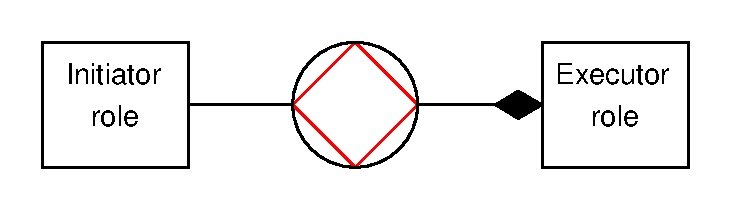
\includegraphics[width=6cm, keepaspectratio]{img/ocd-symbol-example}
    \caption{The core OCD element - transaction symbol with assigned actor roles}
    \label{fig:ocd-symbol-example}
\end{figure}

The PM is in between CM and the AM, that means it is more detailed than CM but less than AM. The PM and the FM are on the same layer of the pyramid and it refers to the fact, that PM takes the process view of coordination world, and the FM is for the production world in the same meaning as PM.

From the CM is used \gls{ocd} which takes standard process pattern and squeeze it to one symbol with two connected boxes which represent initiator and executor actor roles (see \cref{fig:ocd-symbol-example}).

From the PM is taken \gls{psd} sub-model which describes business processes and the exact way how each transaction is connected with another. Following explanation how \gls{psd} is modelled is from~\cite{dietz-essence-2015}:

\begin{quote}
      The disk of the transaction is stretched horizontally, such that it looks like a sausage. One must imagine that there is an invisible and non-proportional time line from left to right (promise is performed after its request,\dots). Coordination acts and facts are represented by small boxes and disks on the border of the transaction symbol (the sausage). 
      The production act, execute, is represented by a small grey box on the edge of the production symbol. To the left of it is the order phase, and to the right the result phase.
      Between two transactions (the sausages) can be added arrows, either solid or dashed. Solid arrows represent \textit{response links}. Response link means that the act at the arrow point is performed in response to the event at the shaft. Dashed arrow represent \textit{waiting links}. Their meaning is that performing the act at the arrow point must wait for the event at the shaft having occurred. Through ``swim lanes'' the responsibility areas of the actor roles are indicated.
\end{quote}
An example of PSD is shown at \cref{fig:psd-example} which means exactly ``When the transaction T1 (Supply order) is \textit{requested}, as a response, T2 (Tax payment) is also \textit{requested}. After that, T1 can be promised only and only, if T2 is \textit{accepted}. After that T1 can be completed''.

\begin{figure}[ht!]
	\centering
    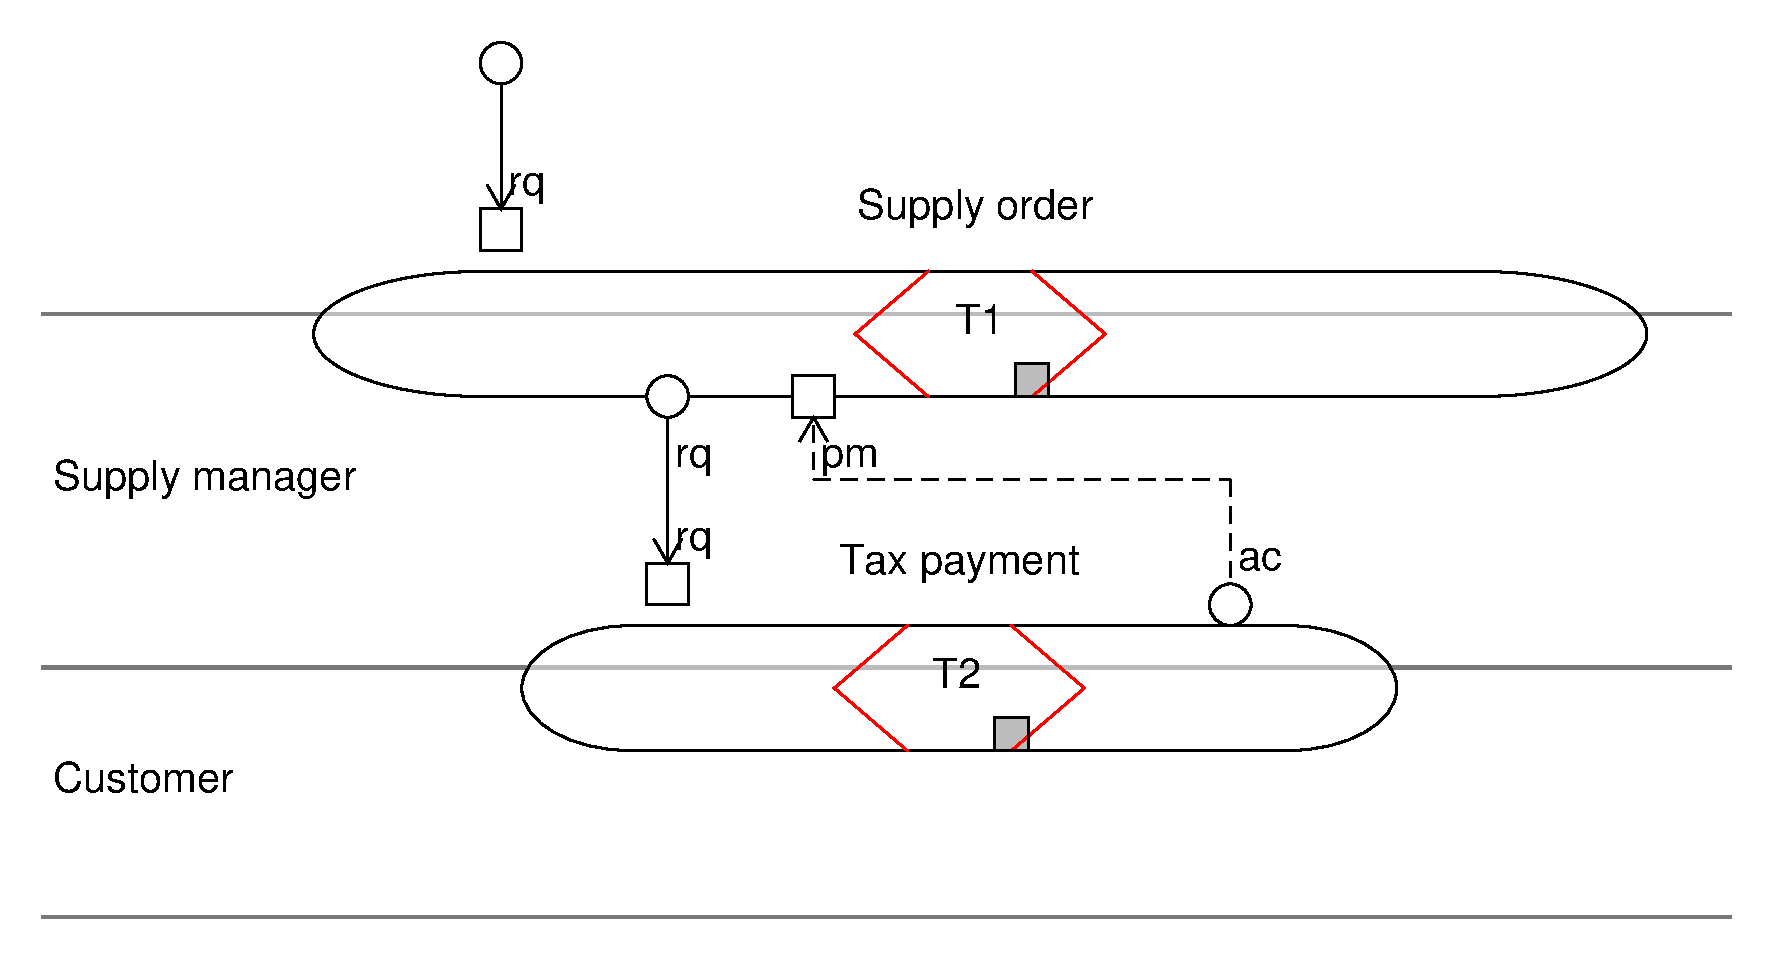
\includegraphics[width=0.7\textwidth]{img/psd-example}
    \caption{PSD example}
    \label{fig:psd-example}
\end{figure}
% -------------------------------------------------------------------------------
\subsection{Advantage of DEMO Over BPMN}    
\gls{bpm} notation is well defined, established and widely used. Many \gls{bpm} solutions exist around and of course, \gls{bpmn} is used ``under the hood''. These systems will be described later in \cref{ch:bpms}.

One thing is absolutely clear, with enlarging business requirements, the business processes "grow up" too and so \gls{bpmn} diagrams. This can lead to very large and complex diagrams, which can be harder to read and understand. One of the advantages of DEMO is the fact, that same \gls{bpmn} diagram can be represented within DEMO notation. The result is reduced complexity with the same understanding as diagram within \gls{bpmn}. However, advantages of DEMO notation can be used not only within \gls{bpmn}. For example, students at subject MI-MEP (Modelling economic processes, translated) at \gls{ctu}~\cite{ccmi-2018} transferred large Trump's flow chart\cite{quartz-trump-2017} (about highway building process) to DEMO OCD diagram. The flow chart that fills several pages, \gls{demo}'s \gls{ocd} fills only one page of size A4. 
To summarize, DEMO can really help to better understand business processes without too much complexity of diagrams itself.
% -------------------------------------------------------------------------------
\section{Gantt chart}
According to~\cite{gantt-chart-2018}, Gantt chart was proposed in 1890 by Karol Adamiecki, but he did publish his work only in the Polish language. About the year 1910 American engineer, Henry Gantt, introduced his own version of this chart and this work became widely used and is still used by project managers. 
Gantt chart serves as an overview of activities according to the time schedule. By simplicity, Gantt chart shows, what has to be done (an activity) and when.
At \cref{fig:gantt-chart-example} is an example of Gantt chart. The core element is some kind of bar chart (progress bar) which starts at some time and is scheduled to end in another time.
Nowadays, Gantt charts, has more advanced elements, such as connected activities (one activity must end before another can start), groups of activities, different colours of activities that can indicate different phases of completion and so on. Many systems for time-management support these types of graphs.
Gantt chart and its usage for this thesis are discussed later, in chapter \cref{ch:proposed-approach}.

\begin{figure}[ht!]
	\centering
    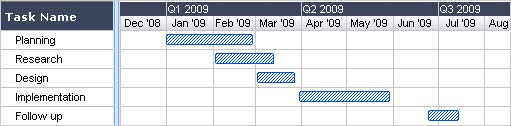
\includegraphics[width=0.8\textwidth]{img/gantt-chart-example.jpg}
    \caption{Gantt chart example \cite{gantt-chart-2018}}
    \label{fig:gantt-chart-example}
\end{figure}



\chapter{Proposed approach}
\todo{Concept art of gantt charts and relations with DEMO}

The main goal of the thesis is to propose a concept of the mobile application which will be able to create the overview of critical business data and make decisions based on them. The concept is kept simple as possible and straightforward to achieve the goals. This chapter will describe each part of the concept and all conceptual features and functions. This chapter is divided to four parts:	
    \begin{enumerate}
      \item Which kind of data the application collects and how it works with them.
      \item What kind of overviews the application can display and how they are connected to the data.
      \item How real-time process visualization is done and how it communicates with internal business systems.
      \item And in the end, the concept of mobile application itself. The screens, supporting systems,\dots \todo{better}.
    \end{enumerate}
    
    \section{Business data}
    
    \subsection{Domain model}    
      \begin{figure}[ht!]
        \centering
        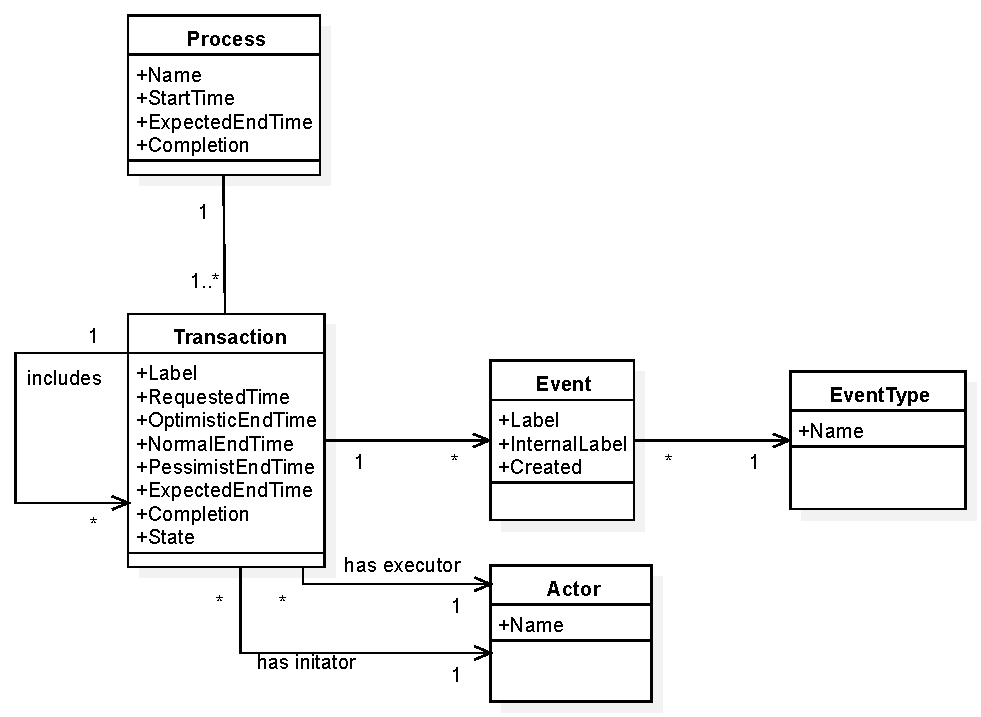
\includegraphics[width=12cm,keepaspectratio]{img/domain-core-model}
        \caption{Domain model \todo{change this image}}
        \label{fig:domain-core-model}
      \end{figure}    
      
      Figure \ref{fig:domain-core-model} shows domain model which describes how collected business data will be transformed for use in mobile application inside overviews and process visualization. 
    
    \section{Overviews}
    
    \section{Process visualization}
    
    \section{Mobile application concept}
	
	\todo{Domain model of collected data. Proposed way of real time visualization. Type of charts. Dashboard. Whole concept of application, e.g dashboard, editor. Functional specification, a.k.a example use cases?? Domain model of collected data.}
% 	\section{Functional specification \todo{Maybe Example use cases}}    
%    \gls{dwma} is mobile-based application that allows managers to create reports over business data. DWMA allows create many types of overviews, such as graphs, that exposing critical information about running business processes. Second critical function is real-time based graph which displays current state of one concrete instance of business process. 
    
% 	This specification  is not complete and focuses only what end-user of \gls{dwma} can do. Spec does not discussed any "deeper" algorithms and used technologies at background.
% Also provided screens and any graphic assets are not final. They only serves as better overview of discussed scenarios, because ``A picture is worth a thousand words".

% 	\todo{Info about RAC - insert whole description of RAC?}. 
    
%     \begin{figure}[h]
%           \centering
%           
\includegraphics{img/TODO-image}
%           \caption{\todo{OCD RAC}}
%       \end{figure}   
    
    
% 	\subsection{Scenario 1 - Janno, one of the CEOs}    
%     Janno is one of the two twins and founders of the \gls{rac} company. He use \gls{dwma} every day mainly for ``top-level" overview of company. He created widget about total amount of request for new car rents at the moment. Also he has a widget which displays number of new requests per day for the last week. Beside this widgets he also created widget where is displayed amount of successfully completed process towards quitted requests grouped by weeks.
    
%     Of course Janno is very wondered about his employees and their productivity. For this purpose, he has a couple more widgets on his dashboard. First is pie chart where every employee from distribution department is displayed with percentages for requests-state acts. Second chart displays number of succeeded requests (request was stated and accepted) at the main office for new rental contracts sorted by from highest to lowest and grouped by employee.
   
%    And one of the important indication of successful company is income, outcome and profit. For this Janno has a widget with simple numbers for each indicators.  
   
    
%     \subsection{\todo{Scenario 2}}   
    
    \section{Analysis}    

   

	\section{The dashboard}
    Purpose of dashboard is provide centralized overview of processes such as average waiting time before process is completed or total amount of requests per day. The appearance of dashboard depends on user. \gls{dwma} provides customizable elements called widgets to achieve desired look for every user individually.

    \subsection{Widgets}  
     Widgets are small independent configurable components for displaying collected data from business processes. Each one has purpose. Notice that widgets are only user-friendly view of query above collected data. For editing widgets there is widget editor. User can simply edit properties of widget such as name, category, tags and of course source of data - the query and second important property is the type of widget. There are following types of widgets:
     
     \textbf{The summary widget} (\cref{fig:widget-summary}) provides, by it's name, chart with summarization of collected data. Concrete type of the chart depends on the user and on the data. Summary widget provides several types of charts:
     
     \begin{enumerate}
    	\item \textit{Pie} chart is used to illustrate numerical proportion.         
        \item  \textit{Bar} chart displays categorical data with numerical value.
        %\item \textit{Line}
    \end{enumerate}
      
      \begin{figure}[ht!]
          \centering
          
\includegraphics[width=6cm,keepaspectratio]{img/TODO-image}
          \caption{Summary widget example}
          \label{fig:widget-summary}
      \end{figure}   
    
   	Second type is \textbf{Time period} (\cref{fig:widget-time-period}). Time period displays data in some interval. Typically it can serve as overview \textit{``Number of requests for Rental payment per day"}.        
      
      \begin{figure}[ht!]
          \centering
          
\includegraphics[width=6cm,keepaspectratio]{img/TODO-image}
          \caption{Time period widget example}
          \label{fig:widget-time-period}
      \end{figure}
    
    Last type is \textbf{Single query} (\cref{fig:widget-single-query}) which allows display simple result from query. Prerequisite for query is that query returns one single record. 
      
      \begin{figure}[ht!]
          \centering
          
\includegraphics[width=6cm,keepaspectratio]{img/TODO-image}
          \caption{Single query example}
           \label{fig:widget-single-query}
      \end{figure}       
    
    \subsection{Query editor}
    
    \todo{Information about query editor}
    
    \begin{figure}[ht!]
          \centering
          
\includegraphics[width=6cm,keepaspectratio]{img/TODO-image}
          \caption{\todo{Query editor}}
      \end{figure}   
    
    \section{The real-time overview of process instance}
    \todo{Introduction about gantt chart. Make conversation about classic OCD / PSD diagrams and their pros and cons for visualizations}
    Provides the real-time overview of one concrete process instance.
On the left side is tree-view (like in folder explorer) of transactions. Each transaction has identifier and name.
On the top is the timeline which displays important events from the process. Above timeline is visualization itself. Each transaction is displayed as progress bar with some visual tweak, which will be discussed later.

	Each transaction can be at one of the following state, which has different visual: 
	\todo{Categories}
    
    \begin{description}
    	\item[Not active transaction] Is displayed as greyed out progress bar. It means that this instance of transaction will be probably started at some future time.

        \item[Active transaction] Progress bar is displayed with green colour to show current progress of instance transaction. 
        
        \item[Completed transaction] Progress bar is fulfilled with green colour. It means that given transaction successfully ended (was accepted).
        
        \item[Stopped transaction]. Progress bar changed colour to red which indicates that transaction failed to complete due to fact that it was quitted or stopped. 
    \end{description}
    
    \subsection{Response and waiting links}
    \todo{Change this}
   Each transaction can have several child-transactions and also many conditional links. These conditions are displayed with arrows pointed to another transaction with the condition.
Conditions are divided into two categories.

If the condition is ``Some state of transaction A has to be done before transaction B can start (be requested)", e.g. transaction A must be stated before transaction B can be requested (\cref{fig:request-start-condition}).

	 \begin{figure}
          \centering
          
\includegraphics[width=6cm,keepaspectratio]{img/TODO-image}
          \caption{\todo{Request-start condition}}
          \label{fig:request-start-condition}
      \end{figure}  

If condition is ``Some state of transaction A has to be done before transaction B can be at another state", e.g transaction A must be at least stated before transaction B can be promised (\cref{fig:state-state-condition}).

	 \begin{figure}
          \centering
          
\includegraphics[width=6cm,keepaspectratio]{img/TODO-image}
          \caption{\todo{State-state condition}}
           \label{fig:state-state-condition}
      \end{figure}  


\chapter{Implementation of concept}

\begin{conclusion}
	%sem napište závěr Vaší práce
\end{conclusion}

\bibliographystyle{iso690}
\bibliography{myref.bib}

\appendix

\printglossaries

\chapter{Content of enclosed CD}

%upravte podle skutecnosti

\begin{figure}
	\dirtree{%
		.1 readme.txt\DTcomment{stručný popis obsahu CD}.
		.1 exe\DTcomment{adresář se spustitelnou formou implementace}.
		.1 src.
		.2 impl\DTcomment{zdrojové kódy implementace}.
		.2 thesis\DTcomment{zdrojová forma práce ve formátu \LaTeX{}}.
		.1 text\DTcomment{text práce}.
		.2 thesis.pdf\DTcomment{text práce ve formátu PDF}.
		.2 thesis.ps\DTcomment{text práce ve formátu PS}.
	}
\end{figure}

\end{document}
